\Exercise
\label{Ex:interpolacio}

Considereu a $\mathbb{R}^2$ els punts $P_0=(1,2)$, $P_1=(2,5)$, $P_2=(3,7)$ i $P_3=(4,3)$ i els vectors $\overrightarrow{P_0'}=(-1,2)$ i $\overrightarrow{P_1'}=(2,-5)$

\begin{enumerate}
  \item Doneu en cada cas la interpolació lineal que passa pels punts
  \begin{enumerate}
    \item $P_0$ i $P_1$
    \item $P_1$ i $P_2$
    \item $P_2$ i $P_3$
    \item $P_0$, $P_1$ i $P_2$ (a trossos)
  \end{enumerate}
  \item Doneu l'spline cúbic d'Hermite que passa pels punts:
  \begin{enumerate}
    \item $P_0$ i $P_1$ amb direccions $\overrightarrow{P_0'}$ i $\overrightarrow{P_1'}$, respectivament
    \item $P_0$ i $P_1$ amb direccions $\overrightarrow{P_1'}$ i $\overrightarrow{P_0'}$, respectivament
    \item $P_1$ i $P_2$ amb direccions $\overrightarrow{P_0'}$ i $\overrightarrow{P_1'}$, respectivament
    \item $P_0$ i $P_1$ amb direccions $\overrightarrow{P_1'}$ i $\overrightarrow{P_0'}$, respectivament
    \item $P_0$ i $P_1$ amb direccions $\overrightarrow{P_0P_2}$ i $\overrightarrow{P_1P_3}$, respectivament
  \end{enumerate}
  \item Doneu l'spline cúbic de Béziers que:
  \begin{enumerate}
    \item Passa per $P_0$ i $P_3$ amb punts de control $P_1$ i $P_2$
    \item Passa per $P_0$ i $P_2$ amb punts de control $P_1$ i $P_3$
    \item Passa per $P_2$ i $P_3$ amb punts de control $P_0$ i $P_1$
    \item Passa per $P_1$ i $P_2$ amb punts de control $P_0$ i $P_3$
  \end{enumerate}

\end{enumerate}

\Answer Considerem cada cas en particular.

\begin{enumerate}

  \item Doneu en cada cas la interpolació lineal que passa pels punts (els resultats globals són graficats a la Figura \ref{fig:interpolaciolineal}):

\begin{enumerate}

  \item interpolació lineal que passa pels punts $P_0$ i $P_1$

Hem de construir una línea recta que passi pels punts $P_0$ i $P_1$. Per a fer-ho, l'estratègia més simple és copnstruir l'equació contínua de la recta. En aquest cas, podem considerar que la recta passarà pel punt $P_0=(1,2)$ i que tindrà com a vector director $\overrightarrow{P_0P_1}=(1,3)$. Per tant:
\begin{equation}
\frac{x-1}{1}=\frac{y-2}{3}
\end{equation}
Quedant $y=\frac{3}{1}(x-1)+2$ a l'intèrval $x\in[1,2]$
\blacksquare

  \item interpolació lineal que passa pels punts $P_1$ i $P_2$

  En aquest cas, podem considerar que la recta passarà pel punt $P_1=(2,5)$ i que tindrà com a vector director $\overrightarrow{P_1P_2}=(1,2)$. Per tant:
  \begin{equation}
    \frac{x-2}{1}=\frac{y-5}{2}
  \end{equation}
  Quedant $y=\frac{2}{1}(x-2)+5$ a l'intèrval $x\in[2,3]$
  \blacksquare

  \item interpolació lineal que passa pels punts $P_2$ i $P_3$

  En aquest cas, podem considerar que la recta passarà pel punt $P_2=(3,7)$ i que tindrà com a vector director $\overrightarrow{P_2P_3}=(1,-4)$. Per tant:
  \begin{equation}
    \frac{x-3}{1}=\frac{y-7}{-4}
  \end{equation}
  Quedant $y=\frac{-4}{1}(x-3)+7$ a l'intèrval $x\in[3,4]$
  \blacksquare

  \item interpolació lineal que passa pels punts $P_0$, $P_1$ i $P_2$ (a trossos)

  Aquí només cal construir una funció a trossos amb els fragments obtinguts abans:
  \begin{equation}
    y= \begin{cases}
           \frac{3}{1}(x-1)+2 , x \in [1,2]\\
           \frac{2}{1}(x-2)+5 , x \in (2,3]
          \end{cases}
  \end{equation}
  \blacksquare

% veure https://tex.stackexchange.com/questions/124346/latex-error-not-in-outer-par-mode

  \begin{minipage}[t]{\linewidth}
    \vspace{-2ex}
    \includegraphics[width=\textwidth]{../figures/interpolaciolineal.pdf}
    \captionof{figure}{Gràfic resum de les respostes a l'exercici. En gris, les rectes resultats, i en negre, els segments d'aplicació de cada interpolació}
    \label{fig:interpolaciolineal}
  \end{minipage}

% \begin{figure}
%     \includegraphics[width=0.5\textwidth]{figures/interpolaciolineal.pdf}
% %    \caption{Gràfic resum de les respostes a l'exercici. En gris, les rectes resultats, i en negre, els segments d'aplicació de la interpolació}
% \end{figure}

\end{enumerate}
\item Doneu l'spline cúbic d'Hermite que passa pels punts donats (els resultats globals són graficats a la Figura \ref{fig:interpolaciohermite}). El polinomi d'Hermite per a una interpolació cúbica es construeix fent $Q_0(t)=T\cdot M \cdot G$ on:
\begin{eqnarray*}
  T&=& \begin{pmatrix}t^3 & t^2 & t & 1\end{pmatrix}\\
  M&=& \begin{pmatrix}
              2 & -2 & 1 & 1 \\
              -3 & 3 & -2 & -1 \\
              0 & 0 & 1 & 0 \\
              1 & 0 & 0 & 0
        \end{pmatrix}\\
  G&=& \begin{pmatrix}
              P_0 \\
              P_1 \\
              P'_0 \\
              P'_1
        \end{pmatrix}\\
\end{eqnarray*}

o bé:
\[
  Q_0(t)=(2t^3-3t^2+1)P_0+(-2t^3+3t^2)P_1+(t^3-2t^2+t)P'_0+(t^3-t^2)P'_1
\]

\begin{enumerate}
  \item $P_0$ i $P_1$ amb direccions $\overrightarrow{P_0'}$ i $\overrightarrow{P_1'}$, respectivament

  \[
    Q_0(t)=\begin{pmatrix}x(t)\\y(t)\end{pmatrix}=(2t^3-3t^2+1)\begin{pmatrix}1\\2\end{pmatrix}
          +(-2t^3+3t^2)\begin{pmatrix}2\\5\end{pmatrix}
          +(t^3-2t^2+t)\begin{pmatrix}-1\\2\end{pmatrix}
          +(t^3-t^2)\begin{pmatrix}2\\-5\end{pmatrix}
  \]
  o bé
  \begin{eqnarray*}
    x(t)&=&(2t^3-3t^2+1)+2(-2t^3+3t^2)-(t^3-2t^2+t)+2(t^3-t^2)\\
    y(t)&=&2(2t^3-3t^2+1)+5(-2t^3+3t^2)+2(t^3-2t^2+t)-5(t^3-t^2)
  \end{eqnarray*}
  Simplificant, obtenim:
  \begin{eqnarray*}
    x(t)&=&-t^3+3t^2-t+1\\
    y(t)&=&-9t^3+2t+2
  \end{eqnarray*}
  \blacksquare



  \item $P_0$ i $P_1$ amb direccions $\overrightarrow{P_1'}$ i $\overrightarrow{P_0'}$, respectivament

  \[
    Q_0(t)=\begin{pmatrix}x(t)\\y(t)\end{pmatrix}=(2t^3-3t^2+1)\begin{pmatrix}1\\2\end{pmatrix}
          +(-2t^3+3t^2)\begin{pmatrix}2\\5\end{pmatrix}
          +(t^3-2t^2+t)\begin{pmatrix}2\\-5\end{pmatrix}
          +(t^3-t^2)\begin{pmatrix}-1\\2\end{pmatrix}
  \]
  o bé
  \begin{eqnarray*}
    x(t)&=&(2t^3-3t^2+1)+2(-2t^3+3t^2)+2(t^3-2t^2+t)-(t^3-t^2)\\
    y(t)&=&2(2t^3-3t^2+1)+5(-2t^3+3t^2)-5(t^3-2t^2+t)+2(t^3-t^2)
  \end{eqnarray*}
  Simplificant, obtenim:
  \begin{eqnarray*}
    x(t)&=&-t^3+2t+1\\
    y(t)&=&-9t^3+17t^2-5t+2
  \end{eqnarray*}
  \blacksquare

  \item $P_1$ i $P_2$ amb direccions $\overrightarrow{P_0'}$ i $\overrightarrow{P_1'}$, respectivament

  \[
    Q_0(t)=\begin{pmatrix}x(t)\\y(t)\end{pmatrix}=(2t^3-3t^2+1)\begin{pmatrix}2\\5\end{pmatrix}
          +(-2t^3+3t^2)\begin{pmatrix}3\\7\end{pmatrix}
          +(t^3-2t^2+t)\begin{pmatrix}-1\\2\end{pmatrix}
          +(t^3-t^2)\begin{pmatrix}2\\-5\end{pmatrix}
  \]
  o bé
  \begin{eqnarray*}
    x(t)&=&2(2t^3-3t^2+1)+3(-2t^3+3t^2)-(t^3-2t^2+t)+2(t^3-t^2)\\
    y(t)&=&5(2t^3-3t^2+1)+7(-2t^3+3t^2)+2(t^3-2t^2+t)-5(t^3-t^2)
  \end{eqnarray*}
  Simplificant, obtenim:
  \begin{eqnarray*}
    x(t)&=&-t^3+3t^2-t+2\\
    y(t)&=&-7t^3+7t^2+2t+5
  \end{eqnarray*}
  \blacksquare

  \item $P_0$ i $P_1$ amb direccions $\overrightarrow{P_1'}$ i $\overrightarrow{P_0'}$, respectivament


      \[
        Q_0(t)=\begin{pmatrix}x(t)\\y(t)\end{pmatrix}=(2t^3-3t^2+1)\begin{pmatrix}2\\5\end{pmatrix}
              +(-2t^3+3t^2)\begin{pmatrix}3\\7\end{pmatrix}
              +(t^3-2t^2+t)\begin{pmatrix}2\\-5\end{pmatrix}
              +(t^3-t^2)\begin{pmatrix}-1\\2\end{pmatrix}
      \]
      o bé
      \begin{eqnarray*}
        x(t)&=&2(2t^3-3t^2+1)+3(-2t^3+3t^2)+2(t^3-2t^2+t)-(t^3-t^2)\\
        y(t)&=&5(2t^3-3t^2+1)+7(-2t^3+3t^2)-5(t^3-2t^2+t)+2(t^3-t^2)
      \end{eqnarray*}
      Simplificant, obtenim:
      \begin{eqnarray*}
        x(t)&=&-t^3+2t+2\\
        y(t)&=&-7t^3+14t^2-5t+5
      \end{eqnarray*}
      \blacksquare


  \item $P_0$ i $P_1$ amb direccions $\overrightarrow{P_0P_2}$ i $\overrightarrow{P_1P_3}$, respectivament

  Primer trobem els vectors:
  \[\overrightarrow{P_0P_2}=P_2-P_0=(3,7)-(1,2)=(2,5)\]
  \[\overrightarrow{P_1P_3}=P_3-P_1=(4,3)-(2,5)=(2,-2)\]

  \[
    Q_0(t)=\begin{pmatrix}x(t)\\y(t)\end{pmatrix}=(2t^3-3t^2+1)\begin{pmatrix}1\\2\end{pmatrix}
          +(-2t^3+3t^2)\begin{pmatrix}2\\5\end{pmatrix}
          +(t^3-2t^2+t)\begin{pmatrix}2\\5\end{pmatrix}
          +(t^3-t^2)\begin{pmatrix}2\\-2\end{pmatrix}
  \]
  o bé
  \begin{eqnarray*}
    x(t)&=&(2t^3-3t^2+1)+2(-2t^3+3t^2)+2(t^3-2t^2+t)+2(t^3-t^2)\\
    y(t)&=&2(2t^3-3t^2+1)+5(-2t^3+3t^2)+5(t^3-2t^2+t)-2(t^3-t^2)
  \end{eqnarray*}
  Simplificant, obtenim:
  \begin{eqnarray*}
    x(t)&=&2t^3-3t^2+2t+1\\
    y(t)&=&-3t^3+t^2+5t+2
  \end{eqnarray*}
  \blacksquare

\end{enumerate}

\begin{minipage}[t]{\linewidth}
  \vspace{-2ex}
  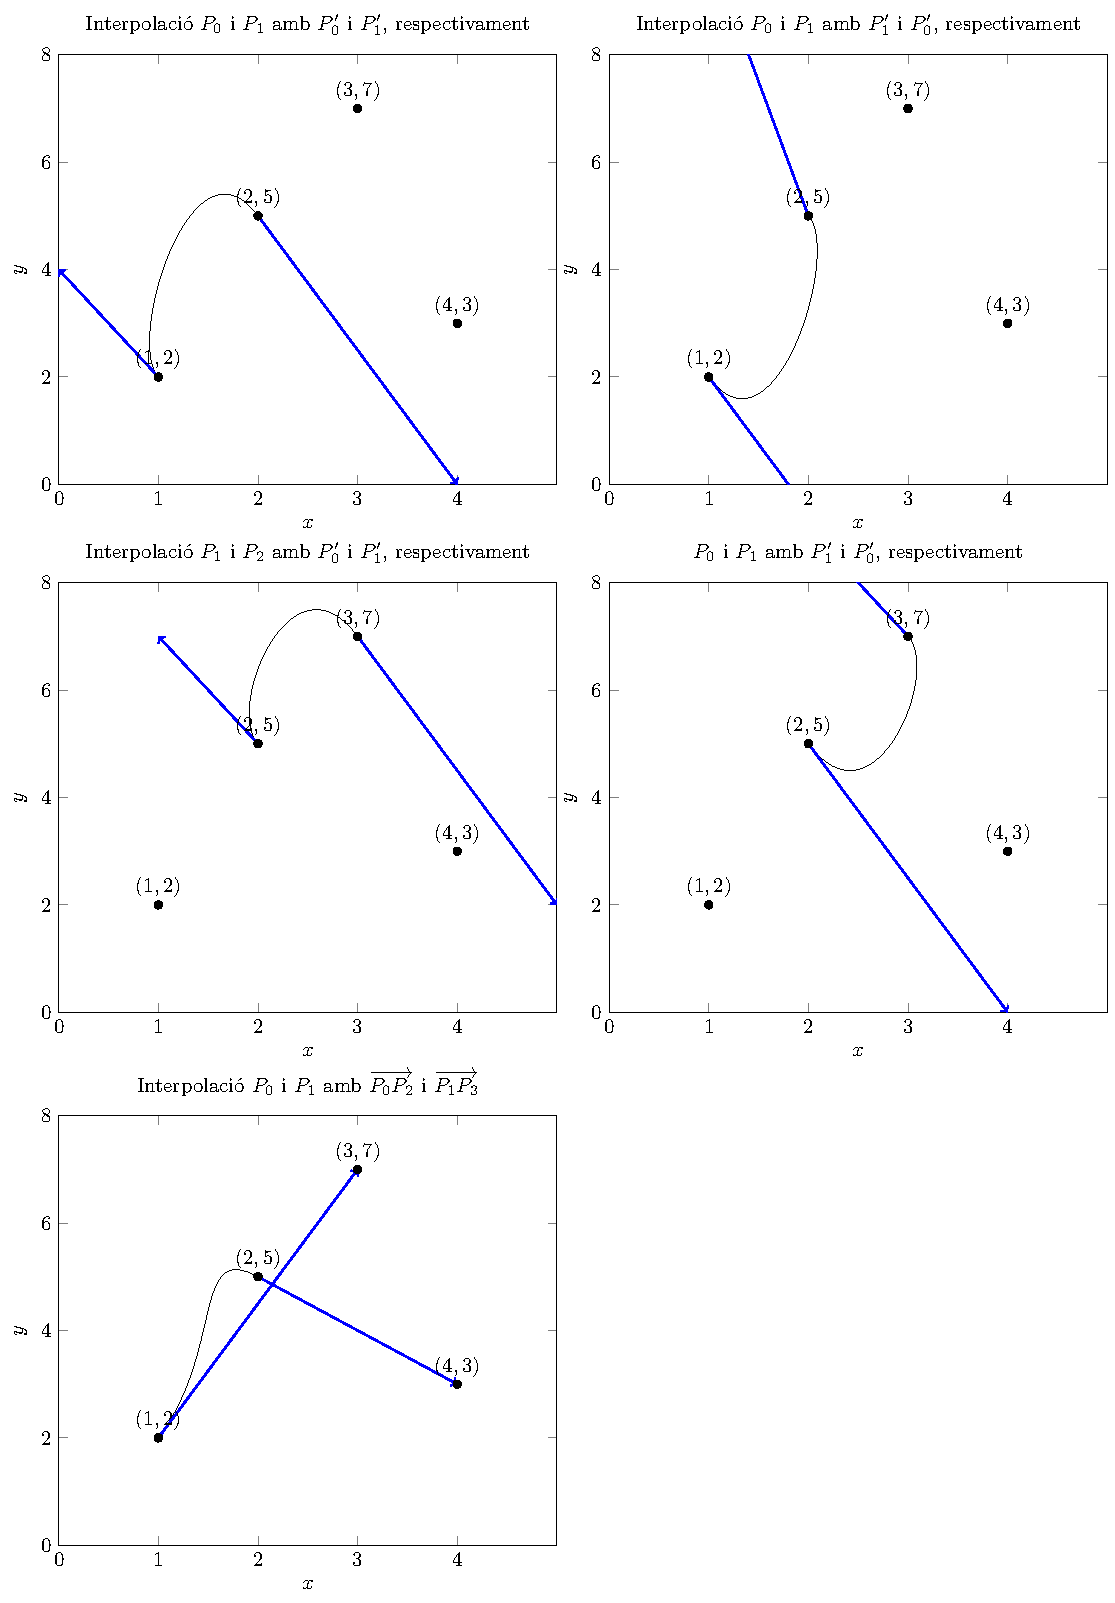
\includegraphics[width=\textwidth]{../figures/interpolaciohermite.pdf}
  \captionof{figure}{Gràfic resum de les interpolacions cúbiques d'Hermite de l'exercici.}
  \label{fig:interpolaciohermite}
\end{minipage}

\item Doneu l'spline cúbic de Béziers que passa pels punts donats (els resultats globals són graficats a la Figura \ref{fig:interpolaciobeziers}). El polinomi de Béziers per a una interpolació cúbica es construeix fent $Q_0(t)=T\cdot M \cdot G$ on:
\begin{eqnarray*}
  T&=& \begin{pmatrix}t^3 & t^2 & t & 1\end{pmatrix}\\
  M&=& \begin{pmatrix}
              -1 & 3 & -3 & 1 \\
              3 & -6 & 3 & 0 \\
              -3 & 3 & 0 & 0 \\
              1 & 0 & 0 & 0
        \end{pmatrix}\\
  G&=& \begin{pmatrix}
              P_0 \\
              P_1 \\
              P_2 \\
              P_3
        \end{pmatrix}\\
\end{eqnarray*}

o bé:
\[
  Q_0(t)=(-t^3+3t^2-3t+1)P_0+(3t^3-6t^2+3t)P_1+(-3t^3+3t^2)P_2+t^3P_3
\]

\begin{enumerate}
  \item Passa per $P_0$ i $P_3$ amb punts de control $P_1$ i $P_2$


  \[
    Q_0(t)=\begin{pmatrix}x(t)\\y(t)\end{pmatrix}=(-t^3+3t^2-3t+1)\begin{pmatrix}1\\2\end{pmatrix}
          +(3t^3-6t^2+3t)\begin{pmatrix}2\\5\end{pmatrix}
          +(-3t^3+3t^2)\begin{pmatrix}3\\7\end{pmatrix}
          +t^3\begin{pmatrix}4\\3\end{pmatrix}
  \]
  o bé
  \begin{eqnarray*}
    x(t)&=&(-t^3+3t^2-3t+1)+2(3t^3-6t^2+3t)+3(-3t^3+3t^2)+4t^3\\
    y(t)&=&2(-t^3+3t^2-3t+1)+5(3t^3-6t^2+3t)+7(-3t^3+3t^2)+3t^3
  \end{eqnarray*}
  Simplificant, obtenim:
  \begin{eqnarray*}
    x(t)&=&3t+1\\
    y(t)&=&-5t^3-3t^2+9t+2
  \end{eqnarray*}


  \blacksquare

  \item Passa per $P_0$ i $P_2$ amb punts de control $P_1$ i $P_3$


      \[
        Q_0(t)=\begin{pmatrix}x(t)\\y(t)\end{pmatrix}=(-t^3+3t^2-3t+1)\begin{pmatrix}1\\2\end{pmatrix}
              +(3t^3-6t^2+3t)\begin{pmatrix}2\\5\end{pmatrix}
              +(-3t^3+3t^2)\begin{pmatrix}4\\3\end{pmatrix}
              +t^3\begin{pmatrix}3\\7\end{pmatrix}
      \]
      o bé
      \begin{eqnarray*}
        x(t)&=&(-t^3+3t^2-3t+1)+2(3t^3-6t^2+3t)+4(-3t^3+3t^2)+3t^3\\
        y(t)&=&2(-t^3+3t^2-3t+1)+5(3t^3-6t^2+3t)+3(-3t^3+3t^2)+7t^3
      \end{eqnarray*}
      Simplificant, obtenim:
      \begin{eqnarray*}
        x(t)&=&-4t^3+3t^2+3t+1\\
        y(t)&=&11t^3-15t^2+9t+2
      \end{eqnarray*}
      \blacksquare

  \item Passa per $P_2$ i $P_3$ amb punts de control $P_0$ i $P_1$

          \[
            Q_0(t)=\begin{pmatrix}x(t)\\y(t)\end{pmatrix}=(-t^3+3t^2-3t+1)\begin{pmatrix}3\\7\end{pmatrix}
                  +(3t^3-6t^2+3t)\begin{pmatrix}1\\2\end{pmatrix}
                  +(-3t^3+3t^2)\begin{pmatrix}2\\5\end{pmatrix}
                  +t^3\begin{pmatrix}4\\3\end{pmatrix}
          \]
          o bé
          \begin{eqnarray*}
            x(t)&=&3(-t^3+3t^2-3t+1)+1(3t^3-6t^2+3t)+2(-3t^3+3t^2)+4t^3\\
            y(t)&=&7(-t^3+3t^2-3t+1)+2(3t^3-6t^2+3t)+5(-3t^3+3t^2)+3t^3
          \end{eqnarray*}
          Simplificant, obtenim:
          \begin{eqnarray*}
            x(t)&=&-2t^3+9t^2-6t+3\\
            y(t)&=&-13t^3+24t^2-15t+2
          \end{eqnarray*}
          \blacksquare

  \item Passa per $P_1$ i $P_2$ amb punts de control $P_0$ i $P_3$


  \[
    Q_0(t)=\begin{pmatrix}x(t)\\y(t)\end{pmatrix}=(-t^3+3t^2-3t+1)\begin{pmatrix}2\\5\end{pmatrix}
          +(3t^3-6t^2+3t)\begin{pmatrix}1\\2\end{pmatrix}
          +(-3t^3+3t^2)\begin{pmatrix}4\\3\end{pmatrix}
          +t^3\begin{pmatrix}3\\7\end{pmatrix}
  \]
  o bé
  \begin{eqnarray*}
    x(t)&=&2(-t^3+3t^2-3t+1)+1(3t^3-6t^2+3t)+4(-3t^3+3t^2)+3t^3\\
    y(t)&=&5(-t^3+3t^2-3t+1)+2(3t^3-6t^2+3t)+3(-3t^3+3t^2)+7t^3
  \end{eqnarray*}
  Simplificant, obtenim:
  \begin{eqnarray*}
    x(t)&=&-8t^3+12t^2-3t+2\\
    y(t)&=&-t^3+12t^2-9t+5
  \end{eqnarray*}
\blacksquare


\end{enumerate}

\begin{minipage}[t]{\linewidth}
  \vspace{-2ex}
  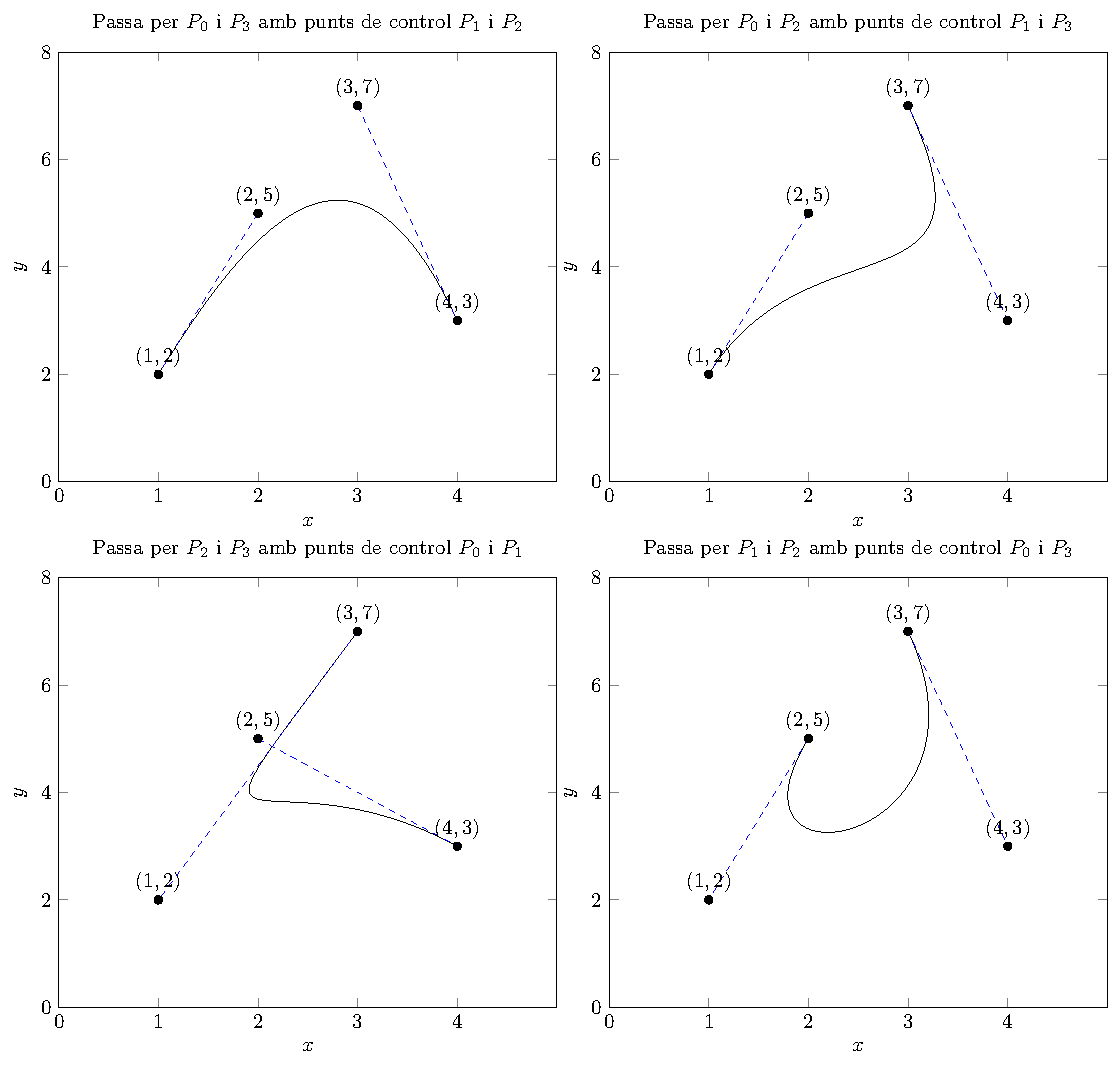
\includegraphics[width=\textwidth]{../figures/interpolaciobeziers.pdf}
  \captionof{figure}{Gràfic resum de les interpolacions cúbiques de Béziers de l'exercici.}
  \label{fig:interpolaciobeziers}
\end{minipage}
Un exemple de codi MATLAB per generar les interpolacions de Beziers pot ser:
\lstinputlisting{../code/polinomisBeziers.m}

\end{enumerate}
